%\begin{headline}[enhanced, tikz={rotate=0}]{Fotios Ptochos Promoted to Professor!}
\begin{headline}[enhanced, tikz={rotate=0}, width=0.48\textwidth]{Fotios Ptochos Promoted to Professor!}
\begin{multicols}{2}
    Congratulations to Fotios Ptochos for his promotion to the rank of
    Full Professor, effective from \MyDate. This promotion recognizes
    Prof. Ptochos' achievements in scholarship, teaching in physics
    and research in high-energy physics (HEP), and his overall service
    to the CDF and CMS Collaborations. He is a Harvard University PhD
    in physics graduate (1998) and has been active in HEP-research
    since 1987. In particular, from 1987 to 1988 he worked in the
    development of a technique to monitor the LAr purity for the first
    ever prototype of the ICARUS detector. From 1989 to 1994 he worked
    in the characterization of various Tetramethyl liquids for the
    envisioned calorimeter detectors at the SSC. He also
    worked in the construction, installation and calibration of the
    CMX system for the CDF detector. From 1994 to 1996 he developed an algorithm to improve
    electron identification for the CDF end-plug ECAL, which led to
    the development and implementation of the PHOENIX tracker system
    in CDF-II.

    In the period of 2000–2003, he was the coordinator of the group
    responsible for the development, installation, maintenance and
    performance monitoring of the CDF-II HCAL timing system. For the entire Tevatron Run-II
    (2001-2011) he served as the coordinator of the CDF central HCAL
    calibration, maintenance and performance group. Since
    2004, when he joined the faculty of the UCY Physics Department, he has
    been involved in the UCY HEP group activities related to the
    construction and running of the CMS ECAL at CERN. In 2009, he
    initiated efforts related to the CMS tracking detector and was
    involved in the development of the dual-readout calorimetry
    concept in a total absorption HCAL for future linear-collider experiments. 

    % ========================
    \begin{figure}
      \begin{center}
        \leavevmode
        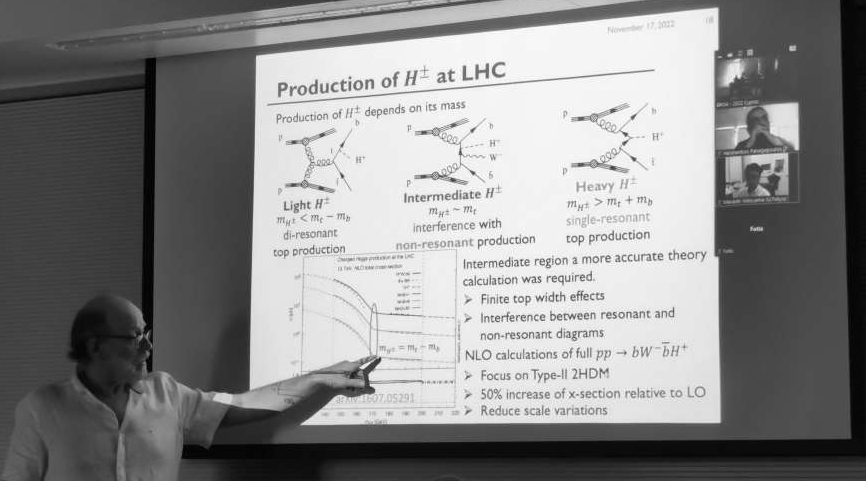
\includegraphics[width=0.4\textwidth]{./figures/Fotis7.png}
      \end{center}
    \end{figure}
    % ========================
%    \begin{wrapfigure}{l}{0.33\textwidth}
%      \begin{center}
%        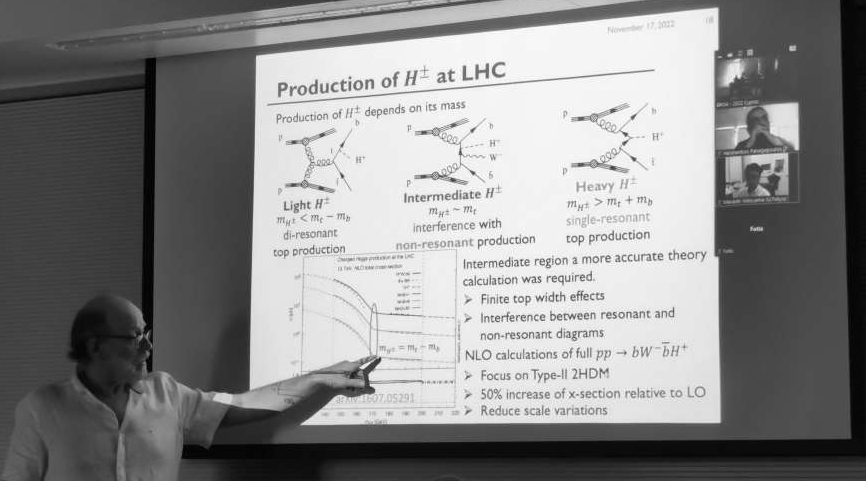
\includegraphics[width=0.22\textwidth]{./figures/Fotis7.png}
%      \end{center}
%      %\caption*{Fotios}
%    \end{wrapfigure}

    Professor Ptochos has led numerous physics analyses, spanning
    from precision measurements on properties of heavy flavour quark
    production and their use as probes for searching for the SM and SUSY
    Higgs bosons, to searches for BSM physics including SUSY, extra
    dimensions and other exotic processes. He has tremendous experience in
    heavy flavour tagging techniques and algorithms, tau-lepton
    identification techniques and new physics model building. 
    He was the first ever recipient of the \say{Fermi National
      Accelerator Laboratory Fellowship} and has co-coordinated multiple research program
    funded primarily by the EC via \textsc{Marie
    Skłodowska-Curie Actions}, the Cyprus RPF through
    \textsc{Didaktor} and \textsc{Excellence Hubs} programs, the ERDF,
    and UCY. He is the author and co-author of more than 
    1850 publications in refereed scientific journals and co-editor of
    education material for the entire Cyprus Secondary Education. He has
    supervised 6 postdoctoral fellows, 5
    PhD and 11 MSc students, as well as projects of more than 20
    undergraduate students.  
\end{multicols}
\end{headline}

